\title{Asymmetric Cryptography - RSA \\
\large SX3007: Mathematical Foundations of Everyday Life}
\date{\today}

\documentclass[11pt]{article}
\usepackage{titling}
\usepackage{multicol}
\usepackage{amsmath}
\usepackage[a4paper, margin=1in]{geometry}
\usepackage{graphicx}
\usepackage{subfig}
\graphicspath{ {./} }

\setlength{\droptitle}{-5em} 
\author{Group Project 1 \\
  Konrad Dryja, 51552177 \\
  Alexandra Riddell, 123 \\
  Danah Alshuaib, 123 \\
  Ogtay Magsudov, 51662109 \\
  Daniel Rennie, 123 \\
  Waleed Totakhyl, 123}
\begin{document}
\maketitle
\begin{multicols}{2}

\paragraph{Introduction}
In the digital age, when majority of our lives and assets is based on virtual systems (such as banking or even entire governments and their elections), it's important to ensure their security from potential threats; those can vary from simple thefts to even foreign states trying to spy on their enemies. To counteract those vectors, we often cipher our messages - normally, we use a shared, secret key, which can be used for both encrypting and decrypting the messages. But the problem of communicating the secret key first remains an issue and potential bottleneck. In order to workaround those shortcomings, we can also apply asymmetric encryption algorithms, where we use two separate entities to encode / decode the message: publicly advertised key and secret, never shared with anyone else, key. One of the example methods being RSA.

\paragraph{Basics of RSA Algorithm}
Let's assume Alice and Bob want to share a message with each other, but don't want Eve to know. There is no secure channel established between A and B, i.e. Eve can freely read the communication between them.

RSA can be applied to choose a public key-pair used for encrypting the messages and a private key which can be used for decryption. To start, Alice would choose two, large prime numbers, $p$ and $q$, their product $p*q \equiv n$ would make a part of the public key. Then, following Euler's totient - calculate the following value $\phi(pq) \equiv (p-1)(q-1)$ along with choosing relatively prime (that is, no number greater than 1 that would divide both numbers) number $e$ to the result - which completes the public key-pair. Now, to compute a private key, we'll have to find a number $d$ such that \(ed \equiv 1 \bmod \phi\), for that calculation, we can use Euler's theorem.

Finally, having obtained both keys, Alice now sends $n$ and $e$ to Bob, keeping $d$ secret. Bob can now encrypt his message by calculating \(c = m^e \bmod n\), where $c$ is the ciphertext and $n$ is the secret message. Then, he sends encrypted message $c$ using insecure channel to Alice. She can then decrypt the message by plugging it into the following formula: $m \equiv c^d \bmod n$


\paragraph{Integer factorization}
RSA is utilizing mathematical problem called integer factorization. Following fundamental theorem of arithmetic, every positive integer can be represented uniquely as a product of primes. For example, number $632$ can be represented as $2*2*2*79 = 2^3 * 79$. Computers nowadays are good with finding out whether a number is prime, but no efficient way has been found to determine prime factors of any (potentially very large) number. Kleinjung et al. was able factor 232 digit number with help of hundred machines in 2 years.\cite{kleinjung2010factorization} Doubling the count increases the time required exponentially. 

\paragraph{HTTPS/TLS}
RSA algorithm nowadays can be found in many places online. One of the best examples is the HTTPS protocol - a green padlock visible on the website, ensuring that connection remains secure. Bank - for example - computes its own private and public key, sharing the latter with a trusted third party. Then, our browser is able to encrypt all outgoing traffic using those keys and send it to the bank, without worrying about anyone eavesdropping. Finally, bank can use their private key to decrypt the message and take relevant action.

\nocite{*}
\bibliographystyle{abbrv}
\end{multicols}

\begin{figure}%
    \centering
    \subfloat[Asymmetric cryptography workflow]{{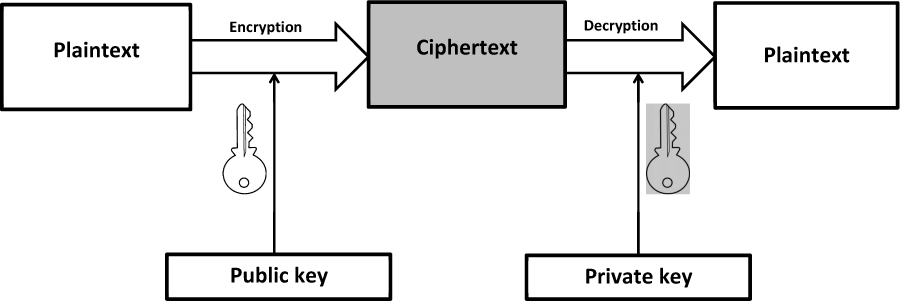
\includegraphics[width=10cm]{example.jpg} }}%
    \qquad
    \subfloat[HTTPS enabled example]{{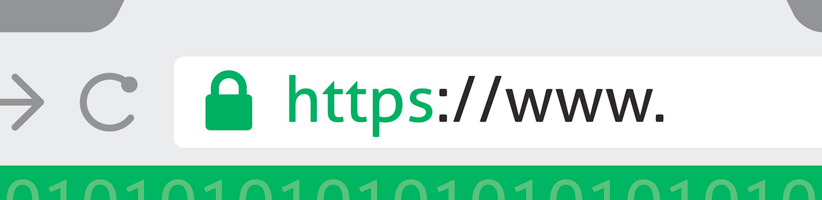
\includegraphics[width=3cm]{https.jpg} }}%
    \label{fig:example}%
  \end{figure}



\bibliography{abstract}
{\huge \textbf{Word count:} 536}
\end{document}

